\documentclass{beamer}
\usepackage{tikz}
\begin{document}
\begin{frame}{After the text}
A first paragraph of text.

A second paragraph.

\begin{tikzpicture}[remember picture, overlay]
  \draw[red] (current page.south west) rectangle (current page.north east);
  \node[anchor=north east, draw] at (current page.north east) {Corner};
\end{tikzpicture}
\end{frame}
\begin{frame}{Before the text}
\begin{tikzpicture}[remember picture, overlay]
  \node[anchor=south west, draw] at (current page.south west) {Low};
\end{tikzpicture}

A first paragraph of text.

A second paragraph.
\end{frame}
\begin{frame}{Within a line}
A first paragraph of text.

\begin{tikzpicture}[remember picture, overlay]
  \node[draw] at (current page.center) {Middle};
  \draw[blue] (0,0) -- (1,1);
\end{tikzpicture}
More text.

A second paragraph.
\end{frame}
\begin{frame}{Between paragraphs}
A first paragraph of text.


\begin{tikzpicture}[remember picture, overlay]
  \draw[blue] (0,0) -- (1,1);
  \node at (2,0) {Local};
\end{tikzpicture}

A second paragraph.
\end{frame}
\begin{frame}[t]{Page coordinates}
A first paragraph of text.

\begin{tikzpicture}[remember picture, overlay, shift={(current page.south west)}]
  \draw[fill=orange!20] (1.2,6.5) rectangle (5.0,8.1);
  \node[anchor=north west, text width=4cm] at (8.3,7.9) {Key result: $x^2$};
\end{tikzpicture}
\end{frame}
\begin{frame}{Not remembered}
Some text here.
\begin{tikzpicture}[overlay]
  \node at (1,0) {Local};
  \node at (current page.center) {Page};
\end{tikzpicture}
\end{frame}
\begin{frame}{In a list}
\begin{itemize}
\item A first item
\item A second 
\begin{tikzpicture}[remember picture, overlay]\node[anchor=west] at (0,0) {Here};\node at (current page.south east) [anchor=south east] {SE};\end{tikzpicture} item
\end{itemize}
\end{frame}
\begin{frame}{In columns}
\begin{columns}
\column{0.5\textwidth}
The left column.
\begin{tikzpicture}[remember picture, overlay]\node[anchor=west] at (0,0) {Origin};\end{tikzpicture}
\column{0.5\textwidth}
The right column.
\end{columns}
\end{frame}
\begin{frame}{In a block}
\begin{block}{Title}
Some body text.

\begin{tikzpicture}[remember picture, overlay]\node[anchor=west] at (0,0) {Inside};\node[anchor=north west] at (current page.north west) {NW};\end{tikzpicture}
\end{block}
\end{frame}
\begin{frame}{Overlays}
Some text.
\only<2>{\begin{tikzpicture}[remember picture, overlay]\node at (current page.center) {Two};\end{tikzpicture}}
\uncover<3>{\begin{tikzpicture}[remember picture, overlay]\node at (current page.north) [anchor=north] {Three};\end{tikzpicture}}
\end{frame}
\begin{frame}{Removed text}
Some text.
\only<2>{X}
\uncover<3>{Y}
\end{frame}
\end{document}
